% Figure 3: Snapshot counts by year (PNG Th1000)
\begin{figure}[H]
\centering
\small
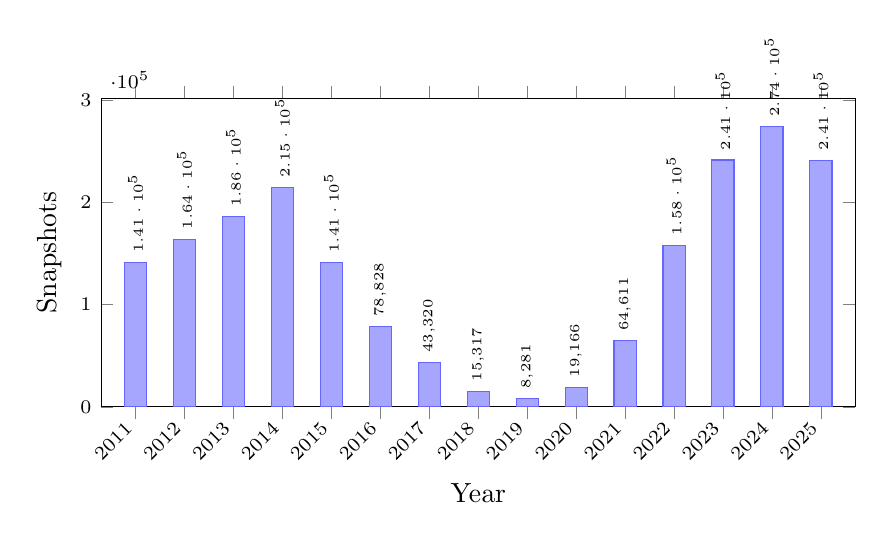
\begin{tikzpicture}
  \begin{axis}[
    ybar,
    bar width=8pt,
    width=0.92\textwidth,
    height=5.5cm,
    ymin=0,
    ylabel={Snapshots},
    xlabel={Year},
    symbolic x coords={2011,2012,2013,2014,2015,2016,2017,2018,2019,2020,2021,2022,2023,2024,2025},
    xtick=data,
    x tick label style={rotate=45, anchor=east, font=\scriptsize},
    y tick label style={font=\scriptsize},
    nodes near coords,
    every node near coord/.append style={font=\tiny, rotate=90, anchor=west},
    enlarge x limits=0.05,
  ]
    \addplot[fill=blue!35, draw=blue!60] coordinates {
      (2011,141005) (2012,164070) (2013,185954) (2014,214503) (2015,141304)
      (2016,78828) (2017,43320) (2018,15317) (2019,8281) (2020,19166)
      (2021,64611) (2022,158002) (2023,241428) (2024,274395) (2025,241063)
    };
  \end{axis}
\end{tikzpicture}
\caption{Number of co-registered magnetogram snapshots per calendar year in the JW-FD release (PNG branch, $B_{\mathrm{th}}=1000$~G). Counts reflect solar-cycle activity: Solar Cycle~24 peak years (2013--2014, 2023--2025) dominate; the 2018--2020 minimum is clearly visible.}
\label{fig:year_chart}
\end{figure}
